\documentclass[tikz, border=1cm]{standalone}
\usepackage{tikz}

\begin{document}
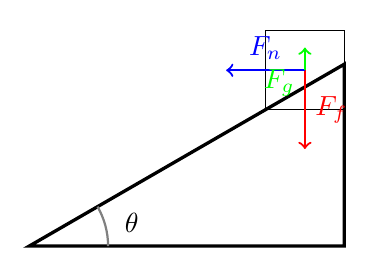
\begin{tikzpicture}

% Define the slope angle
\pgfmathsetmacro{\angle}{30}

% Draw the slope
\draw[very thick] (0,0) -- (4,0) -- (4,{4*tan(\angle)}) -- cycle;

% Draw the block
\draw (3,{3*tan(\angle)}) rectangle ++(1,1);

% Draw and label the forces
\draw[->,red,thick] (3.5,{3*tan(\angle)+0.5}) -- node[right] {${F}_{f}$} (3.5,{3*tan(\angle)-0.5});
\draw[->,blue,thick] (3.5,{3*tan(\angle)+0.5}) -- node[above] {${F}_{n}$} (2.5,{3*tan(\angle)+0.5});
\draw[->,green,thick] (3.5,{3*tan(\angle)+0.5}) -- node[below left] {${F}_{g}$} (3.5,{3.5*tan(\angle)+0.5});

% Draw and label the angle
\draw [gray, thick] (1,0) arc [start angle=0, end angle=\angle, radius=1];
\node at (1.3,0.3) {${\theta}$};

\end{tikzpicture}
\end{document}